\begin{figure}
    \centering
    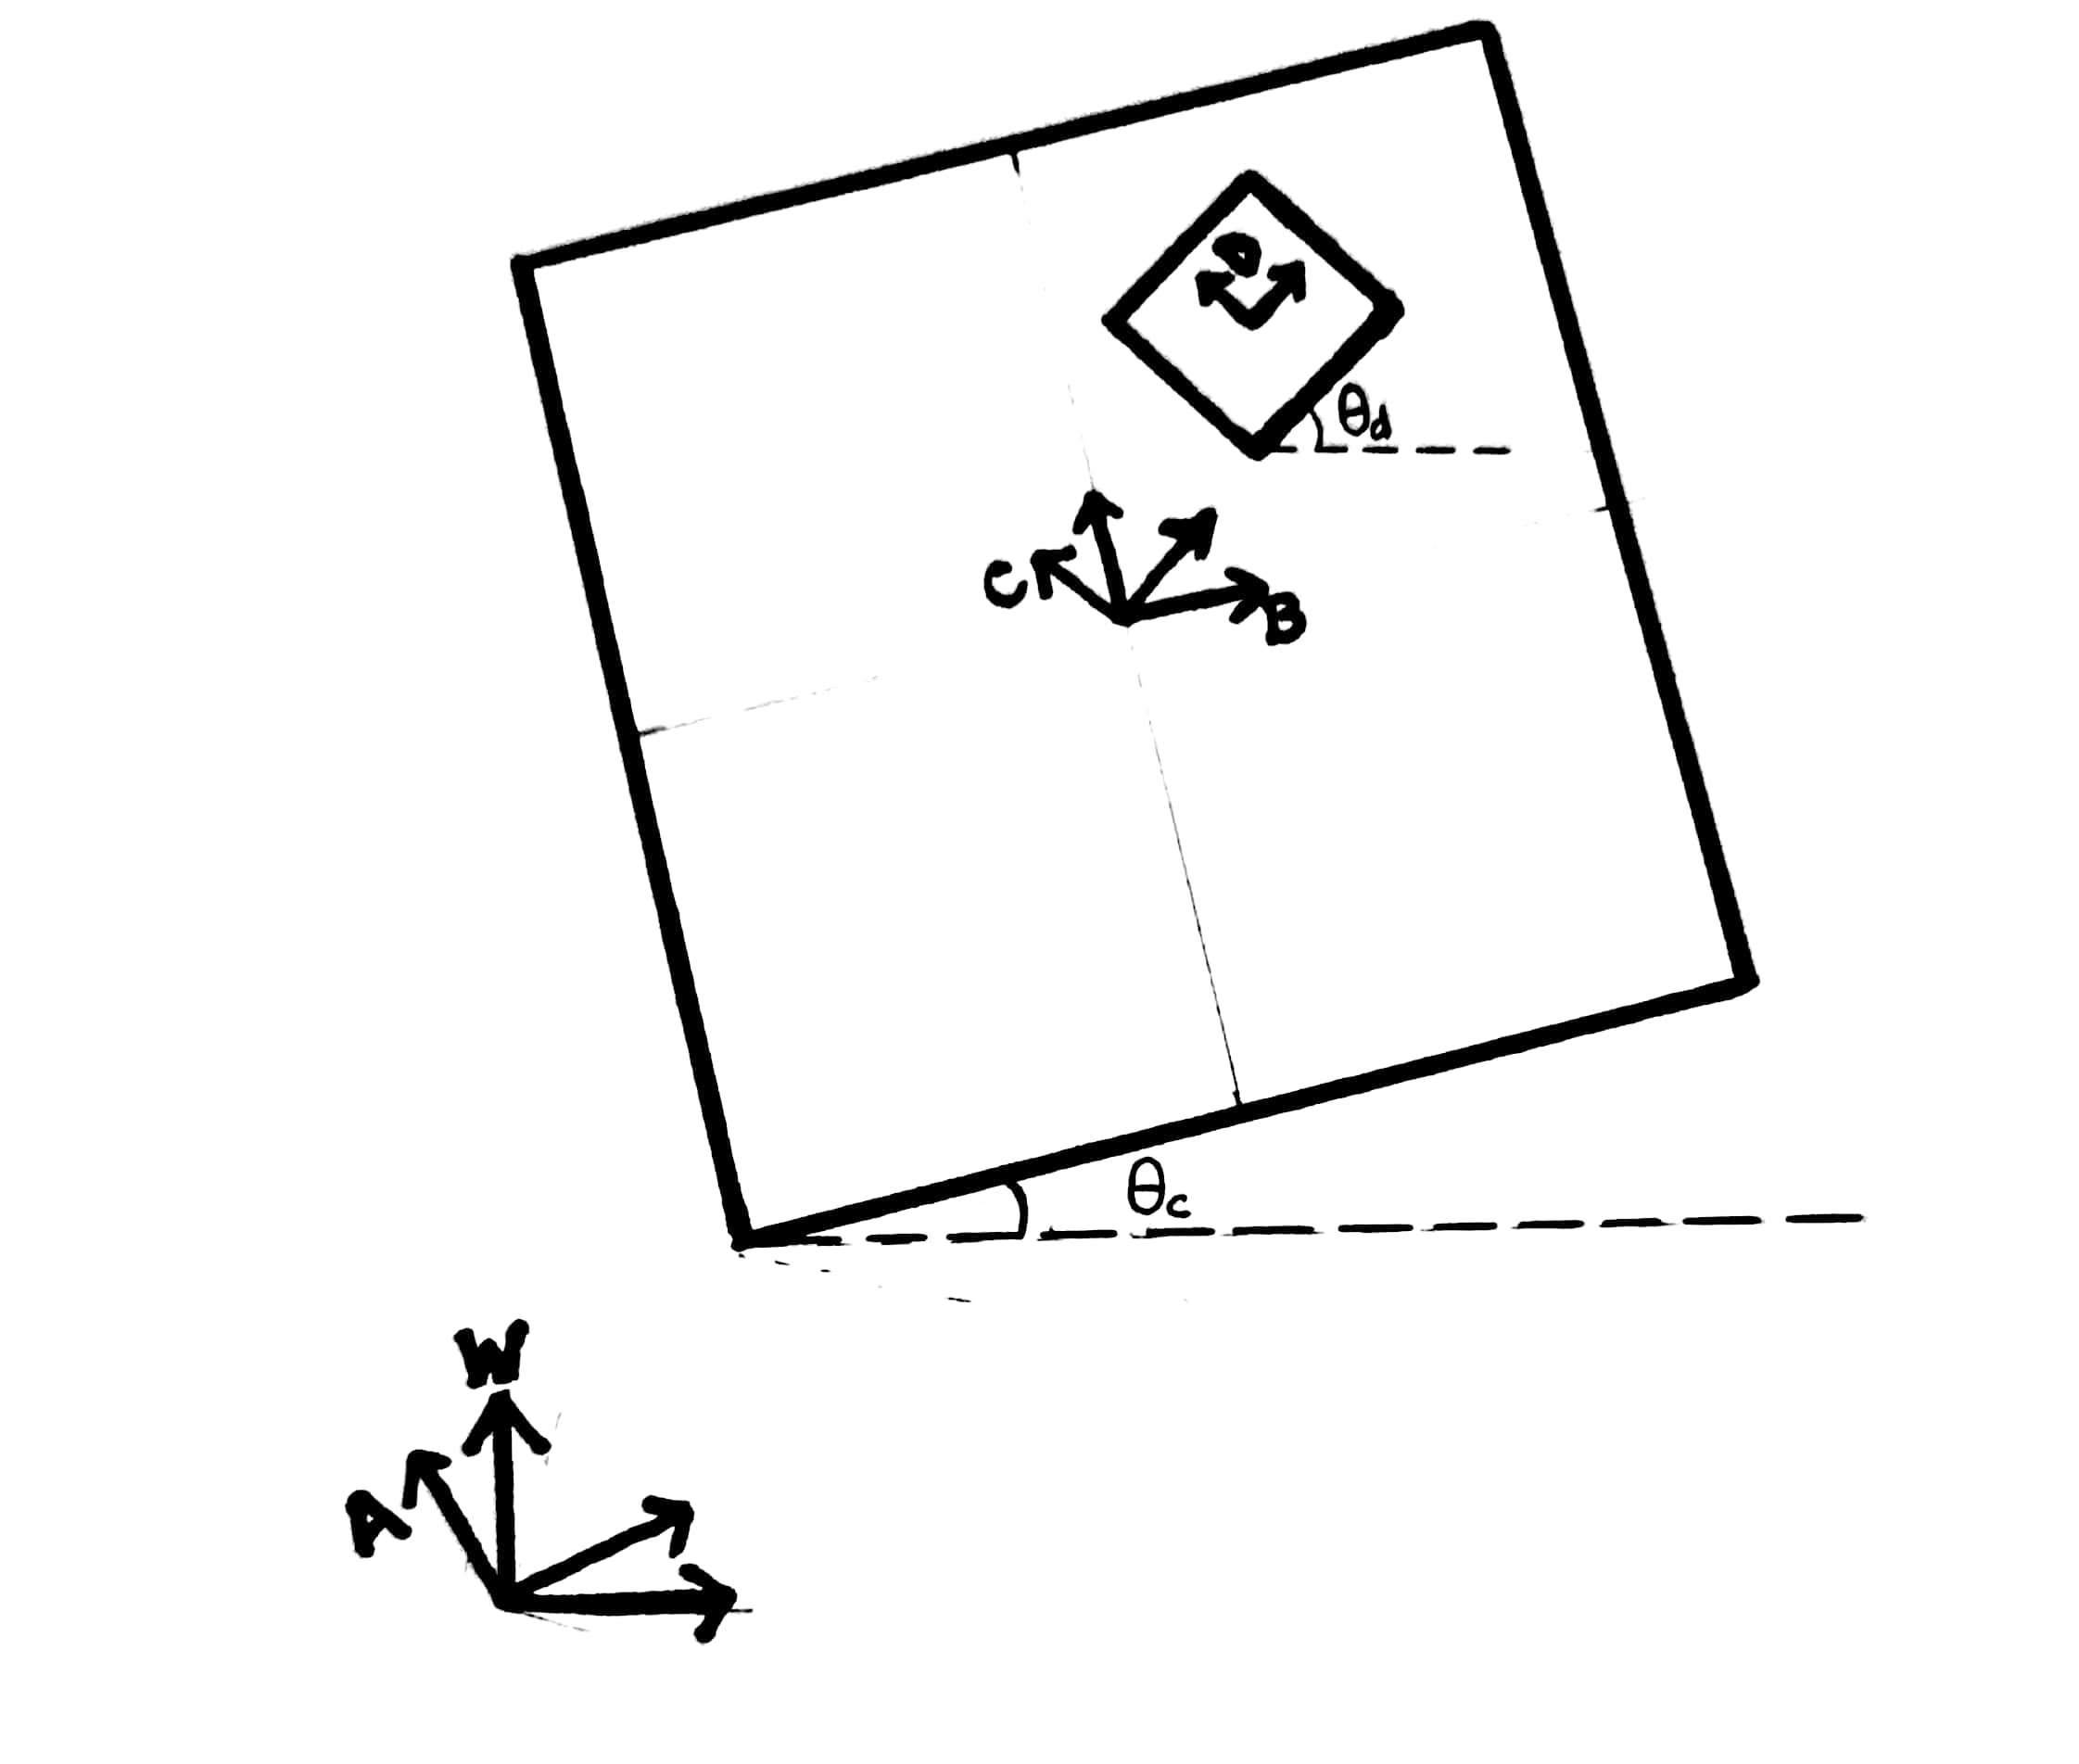
\includegraphics[width=0.75\textwidth]{figs/Diagram.jpg}
    \caption{Diagram of the dice in cup system including coordinate frames}
    \label{diagram}
\end{figure}

\section{Overview}
For the final project, I chose to do the "dice in a cup" problem. This problem was modelled as if you were looking down at a singular die
on a table. A cup is placed over the die and shaken around only in the plane of the table. This means that for this problem we can model the  
die in a cup as a small 2D square (die) in a larger 2D square(cup). With these assumptions, we can ignore gravity since it would point perpendicular
to the surface on which the die and cup are moving. There are 16 possible impacts in this system, which include each vertex of the die 
impacting which each of the four walls. This is assuming we are not considering the unlikely case 
of simultaneous impact where an entire side of the die strikes a wall of the cup at once. Note that at the end of this report, the Python Jupyter notebook 
used to complete this problem as well as a python file with helper functions is shown.

\section{Setup}
First I defined the configuration variables I would need for this system. This inlcuded an x and y coordinate as well as angle measured from the x (horizontal) axis 
in the world frame {W} for both the cup and the die, leaving us with a total of 6 configuration variables.
\begin{equation*}
    q = [x_c, y_c, \theta_c, x_d, y_d, \theta_d,]
\end{equation*}

Next, I defined several frames which are shown and labelled in Figure \ref{diagram}. The world frame is labelled {W}, and this is where we will start and reference
the other frames back to. Next, I defined the A frame to be a counter-clockwise rotation by an angle $\theta_c$. We arrive at Frame {B} by doing a translation by $x_c$ and $y_c$.
Frame B is located a the center of mass of the cup. Finally, we rotate by an angle $\theta_d$ to get to frame {C} and translate by $x_d$ $y_d$ to get to frame {D} which is located at 
the center of mass of the die. If we wanted to, we could define frames at the vertices of the die, however with the orientation of the {D} frame as it is, it is easy enough to define 
the vertices of the die simply in terms of the die's width.

\section{Process}
To achieve the final result shown in the submitted video, I began by defining the coordinate frames and relating them back to the world frame with SE(3) transformations. Next, I went
through the familiar process of computing body velocites, kinetic energy, potential energy (although with our assumptions it is zero), and the Lagrangian. Then I defined an external force
to simulate the shaking of the cup. This was chosen to be a sinusoidal function with an arbitrarily chosen gain term $k$ to make the shaking of the cup appropriate for the animation.
At this point I solved the Euler-Lagrange equations for this system.
\subsection{Impacts}
Arguably the most challenging and time consuming aspect of the project was defining and all the impact conditions and solving the impact equations. To define the impact conditions, I first used
rigid body transformations to get the coordinates of the vertices of the die in the {B} frame (the cup body frame). This allowed me to set impact conditions very easily. For example, for the
top right corner of the die, after getting the coordinates in the {B} frame, I could simply say that the impact with the right wall occured when the x-coordinate of that vertex in the {B} frame 
is equal to half the width of the cup. Likewise, the impact between that point and the bottom of the cup occurs when the y-coordinate of that point in the {B} frame is equal to the minus half 
the width of the cup. This is how I was able to define impacts for all the vertices. 
\paragraph{Simulation}
The impact equations for each of the 16 impacts were too big to solve symbolically with SymPy. Therefore, to solve this issue, I combined the solving of the impact equations with the simulation 
loop. At each time step, I check for an impact, and if there is one, I plug in the current state vector (which is a function of q and qdot) into the appropriate impact equation. This makes for a 
fast solution since many of the terms in the equations just become floats.

\section{Conclusion}
Finally, all this was simulated and can be seen in the attached .mp4 file. The code is in this same PDF following this report. In conclusion, the simluation looks very accurate to what I would 
anticipate it to look like. When the die hits the wall at angle it bounces off an angle consistent with reality. It also seems to spin more or less depending on how it contacts a wall of the cup.
This all happens in a manner that is not suprising to watch and looks just like how I would imagine it happening in real life.

